\chapter{配置應用環境}\label{ch:remote}
\index{Yuancheng jisuan@遠端計算}

完成本地結構和工作流練習後，可以按需要調整介面、連線材料資料庫，或把計算提交給已經配置好的遠端環境。這些功能分別解決不同的問題：設定決定應用如何與個人服務配合，遠端計算決定工作流在哪裡執行，日誌與幫助則用於理解當前狀態並交流問題。

本章先介紹日常使用的設定與對話服務，再介紹完整 MATLAB\regmark{} 工具箱中的遠端提交。節點內的CPU、程序池與GPU設定見第\ref{sec:node-resources}節；本章的遠端部分解決的是把任務交給哪一個計算環境。使用獨立應用或基於 Runtime 的線上版時，可按自己的部署條件使用節點資源，並閱讀設定、對話、日誌與幫助各節。

\section{調整應用設定}

\subsection{開啟設定並儲存修改}

在 \ui{主頁} 的環境區域點選 \ui{設定}。通用頁包含介面語言和對話服務設定，Materials Project 頁用於資料庫訪問；連線賬號服務的線上版環境還提供賬號頁。

更改後點選 \ui{確認} 才會儲存。點選 \ui{取消} 或直接關閉設定視窗，會放棄本次尚未確認的修改。再次開啟視窗時，會重新讀取已經儲存的值，可以據此核對實際採用的設定。

\subsection{切換介面語言}
\index{Jiemian yuyan@介面語言}

\begin{steps}
\item 開啟 \ui{主頁 → 設定 → 通用}。
\item 在語言區域選擇需要的介面語言。
\item 點選 \ui{確認}，儲存選擇。
\item 儲存正在編輯的專案，然後重新啟動應用。
\item 檢查工具欄與面板標題是否已經使用新的語言。
\end{steps}

語言在下次啟動時生效。桌面應用關閉後重新開啟即可；線上版中 \ui{退出 KSSOLV Toolbox} 只是暫時返回入口，原例項仍在執行。線上版使用者需要先儲存專案，再按平臺的登出或重新啟動流程進入新的例項。

圖\ref{fig:settings-language-field}給出線上版通用頁的語言區域區域性。當前選擇為簡體中文，輸入框下方說明語言在下次啟動時生效；這與本節先儲存設定、再重新啟動的操作順序對應。

\begin{figure}[!htb]
\centering
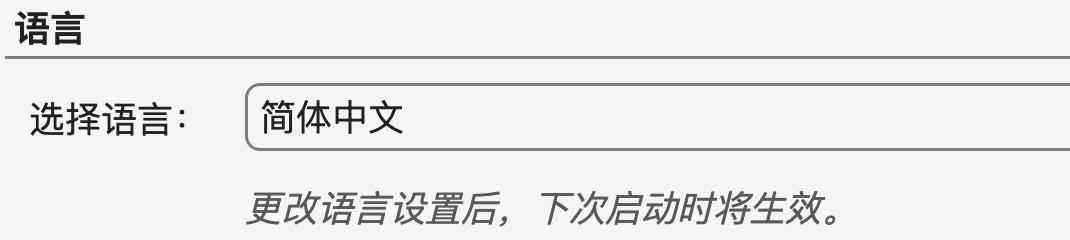
\includegraphics[width=102mm]{publication-assets/crop-290321d16b2310a99270.png}
\caption{設定通用頁的語言欄位例項，當前選擇簡體中文。}
\label{fig:settings-language-field}
\end{figure}


\section{連線對話服務}\label{sec:llm-configuration}
\index{Duihua fuwu@對話服務}

\subsection{選擇服務型別}

命令列視窗除了執行可用命令，還可以向大語言模型提問。應用提供\ui{OpenAICompatible}與\ui{Ollama}兩種服務型別。前者使用OpenAI相容的介面，由服務提供方給出基礎地址、金鑰與模型名稱；後者連線已經執行的Ollama服務，使用該服務已經安裝的模型。

對話適合解釋術語、比較引數的用途和整理工作筆記。支援工具呼叫的模型還可以讀取當前工作流、修改節點標籤。對話服務為可選功能，結構匯入、建模和DFT計算可獨立使用。

\begin{table}[!htb]
\centering
\caption{選擇服務時需要準備的資訊。}
\label{tab:llm-connection-fields}
\begin{tabularx}{\linewidth}{lXX}
\toprule
設定 & OpenAICompatible & Ollama \\
\midrule
地址 & \ui{API 基礎地址}，包括提供方要求的版本路徑，如\file{/v1}。 & \ui{服務地址}，如本機服務的\url{http://127.0.0.1:11434}。\\
憑據 & \ui{API Key}，填寫該基礎地址對應的金鑰。 & 此設定頁不提供API Key欄位。\\
模型 & \ui{使用的模型}，選擇或輸入賬號可用的模型標識。 & \ui{使用的模型}，選擇或輸入服務端已安裝的名稱與標籤。\\
檢查 & \ui{測試連線}或重新整理按鈕獲取模型列表。 & \ui{測試連線}或重新整理按鈕獲取已安裝模型列表。\\
\bottomrule
\end{tabularx}
\end{table}

這裡的地址由執行工具箱的機器訪問。桌面應用通常從桌面計算機發出請求，線上版則由伺服器或容器訪問服務；瀏覽器所在電腦並不自動成為模型服務的執行位置。

\subsection{設定 \headinglatin{OpenAI} 相容服務}

開始前，從服務提供方取得基礎地址、個人 API Key 和有權使用的模型。“OpenAI 相容”表示介面形式，提供方和模型由所用服務決定。

\begin{steps}
\item 在 \ui{主頁 → 設定 → 通用} 中找到\ui{大語言模型}區域，將\ui{型別}設為\ui{OpenAICompatible}。
\item 在 \ui{API 基礎地址} 中輸入提供方給出的基礎地址，保留其要求的版本路徑。
\item 在 \ui{API Key} 中輸入個人金鑰。
\item 點選 \ui{測試連線}，等待獲取模型列表的狀態提示。
\item 從 \ui{使用的模型} 中選擇可用模型，或按提供方說明輸入準確標識，核對名稱後點選 \ui{確認}。
\item 回到命令列視窗，用一個簡短的概念問題檢查服務是否能正常回答。
\end{steps}

圖\ref{fig:settings-service-fields}展示OpenAI相容服務的配置欄位。基礎地址保留提供方要求的版本路徑；模型標識應與服務端可用名稱一致。填寫後，點選\ui{測試連線}獲取模型列表。

\begin{figure}[!htb]
\centering
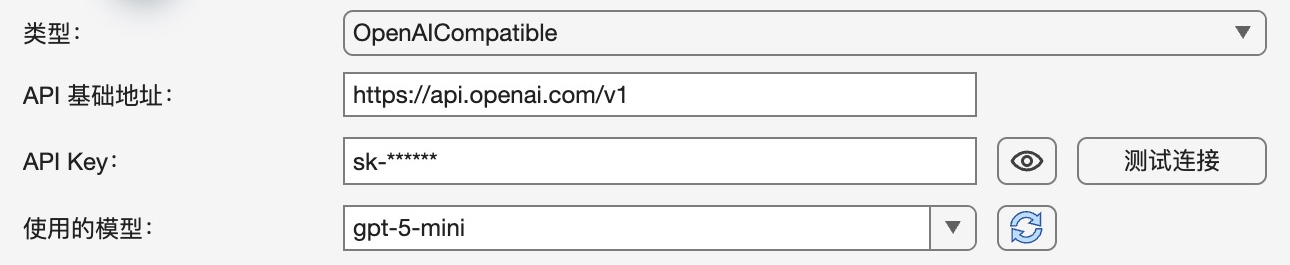
\includegraphics[width=\linewidth]{publication-assets/revision-llm-openai-compatible.png}
\caption{OpenAI相容服務的中文設定頁區域性。基礎地址、金鑰和模型分別填寫；金鑰以遮擋形式顯示。}
\label{fig:settings-service-fields}
\end{figure}

基礎地址應使用提供方給出的API根地址，省略\file{/chat/completions}、\file{/models}等具體介面路徑。例如，提供方要求的基礎地址若以\file{/v1}結束，就應保留這一段；應用隨後會自行追加獲取模型列表或請求回覆的路徑。設定頁會拒絕已經包含上述具體介面路徑的基礎地址。

金鑰輸入框通常以遮擋形式顯示。若需更正可以使用顯示按鈕短暫檢視，完成後恢復隱藏。如需刪除已經儲存的OpenAI金鑰，先選擇另一種不使用它的服務，再清空金鑰並點選\ui{確認}；仍選OpenAI相容服務時，設定頁會要求填寫可用金鑰。截圖或共享螢幕時保持金鑰隱藏。

\subsection{設定 \headinglatin{Ollama}}

Ollama 需要一個已經執行並能由應用訪問的服務。桌面使用者可以使用本機服務，線上版則需使用伺服器能訪問的地址。服務請求由執行工具箱的機器發出。

\begin{steps}
\item 在\ui{型別}中選擇\ui{Ollama}。
\item 在\ui{服務地址}填寫服務根地址，不附加\file{/api/tags}或其他具體API路徑。本機預設埠的地址可寫為\url{http://127.0.0.1:11434}。
\item 點選\ui{測試連線}，等待讀取服務端的模型列表。
\item 在\ui{使用的模型}中選擇服務已經安裝的模型，或輸入完整名稱與標籤，再點選 \ui{確認}。
\item 回到命令列視窗傳送簡短問題，檢查狀態與回覆。
\end{steps}

線上版中的 \file{localhost}或\file{127.0.0.1} 指執行工具箱的伺服器或容器，不能用它指向個人筆記本上的 Ollama。使用統一模型服務時，直接填寫部署方給出的伺服器地址。在列表中填寫模型名稱不會替伺服器下載模型；模型的安裝與服務啟動應先在提供該服務的環境中完成。


\begin{figure}[!htb]
\centering
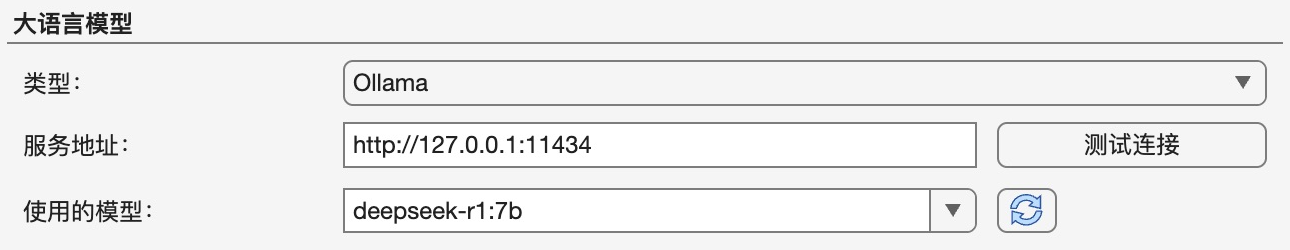
\includegraphics[width=\linewidth]{publication-assets/revision-llm-ollama.png}
\caption{Ollama服務的地址與模型配置。}
\label{fig:llm-ollama-live}
\end{figure}

\subsection{重新整理模型列表}

\ui{測試連線}和模型旁的重新整理圖示執行同一種檢查：向當前地址獲取模型列表。OpenAI相容服務讀取\file{/models}，Ollama讀取\file{/api/tags}。取得非空列表後，狀態顯示\ui{連線成功，已獲取模型}及數量。所選模型的文字回復與工具呼叫能力可在命令視窗中透過提問檢查。

修改地址或金鑰後，先重新整理，再檢查\ui{使用的模型}。測試期間按鈕會改為\ui{停止測試}，點選它可以結束本次等待。模型框允許手動輸入，因此當服務沒有返回可列舉列表、但提供方另給了準確模型名稱時，可以填寫該名稱並儲存，再透過一次簡短提問檢查對話。服務未提供模型列表時，列表測試可能仍提示沒有發現模型。

認證失敗時檢查地址與金鑰是否屬於同一服務；介面不存在時檢查基礎地址及版本路徑；超時或安全連線提示則檢查執行工具箱的機器能否連線該服務。若能取得模型列表但提問失敗，繼續檢查所選模型的使用許可權、對話介面以及工具呼叫支援，而不要只反覆重新整理列表。介面提示本發行包沒有對話元件時，應使用提供相應元件的發行環境；這不會影響本書的結構與DFT教程。

\subsection{在命令視窗提問}\label{sec:chat-use}

對話和普通命令共用一個輸入區，由開頭符號區分。普通MATLAB\regmark{}表示式直接輸入；以一個美元符號開頭表示帶已有對話上下文提問，以兩個美元符號開頭表示本次不帶已有對話歷史。美元符號是輸入的一部分，不需要先切換另一張聊天頁面。

\begin{table}[!htb]
\centering
\caption{同一輸入區中的命令與提問。}
\label{tab:command-chat-prefix}
\begin{tabularx}{\linewidth}{lX}
\toprule
輸入示例 & 實際作用 \\
\midrule
\texttt{2 + 3} & 執行MATLAB\regmark{}表示式，在命令視窗顯示結果。\\
\texttt{\$}後接問題 & 向模型提問，沿用此前成功完成的對話上下文。\\
\texttt{\$\$}後接問題 & 獨立提問，不讀取也不追加此前儲存的對話上下文。\\
\bottomrule
\end{tabularx}
\end{table}

\begin{steps}
\item 在設定中確認服務與模型後，開啟命令列視窗，等待輸入區可用。先輸入\literalinput{2 + 3}並按Enter，識別普通命令的返回位置。
\item 輸入\literalinput{$ 请解释平面波截断能的含义}，按Enter，觀察等待狀態及逐步出現的回覆。
\item 需要繼續追問時，輸入\literalinput{$ 为什么还需要检查k点收敛}，使問題沿用當前對話。
\item 希望獨立詢問另一件事時，輸入\literalinput{$$ 请说明分数坐标的三个分量}。這不會清空前面的對話；下一次單美元符號提問仍可沿用原上下文。
\item 將需要保留的解釋整理到實驗筆記，再回到結構或工作流繼續建模與計算。
\end{steps}

首次提問時，應用才建立所選服務的對話客戶端。傳送後觀察等待狀態與逐步出現的回覆，回覆結束後狀態區可能顯示服務實際返回的模型名稱。正在回覆時，應等這一輪結束再提下一問。

應用可以顯示普通文字、程式碼塊和數學表示式。模型寫出的程式碼只是回覆內容，不會因為顯示在視窗裡便自動執行。需要嘗試其中某條命令時，先核對變數和輸入，再將它作為不帶美元符號的普通命令提交。提問時寫明相關結構、計算條件和數值，便於模型圍繞具體問題回答。


\begin{figure}[!htb]
\centering

\includegraphics[width=108mm]{publication-assets/revision-llm-question-input.png}
\caption{命令視窗中的提問輸入示例。開頭的美元符號區分對話與普通命令；畫面為傳送前狀態。}
\label{fig:llm-input-live}
\end{figure}

\subsection{讓模型檢視並整理當前工作流}\label{sec:chat-workflow-tools}

支援工具呼叫的模型可以請求應用執行兩項操作：讀取當前工作流的節點與連線，以及修改指定節點的標籤。讀取當前流程對應\texttt{getCurrentGraph}；修改標籤對應\texttt{changeNodeLabel}。這兩項工具不負責新建結構、修改計算引數、啟動計算或讀取整個專案的數值結果。

OpenAI相容請求會帶上這兩項工具的定義，服務與模型需要支援相應的工具呼叫格式。Ollama則根據服務報告的模型能力決定是否提供工具；不支援工具的模型仍可進行普通文字對話。工具是否已執行，可結合對話返回內容與畫布變化檢視。

\begin{steps}
\item 儲存當前專案，啟用一張已經建立的工作流，使其成為當前畫布。
\item 輸入\literalinput{$ 请读取当前工作流，说明节点标签和连接顺序}。能夠呼叫工具時，模型可用實際流程資訊組織回答。
\item 檢查回答中的標籤是否與畫布一致。如果回答只是一般說明，明確要求讀取當前工作流；仍沒有實際資訊時，檢查所選模型的工具支援。
\item 選擇一個容易識別的節點，例如當前流程中唯一的SCF節點，再輸入\literalinput{$ 请把当前流程中SCF节点的标签改为“电子自洽”}。若有多個同類節點，在問題中給出原標籤，先確定目標。
\item 返回畫布檢查標籤是否改變，再開啟該節點配置，確認任務仍是SCF。儲存專案以保留這次編輯。
\end{steps}

修改標籤只改變畫布上的名稱，不會把別的任務變成SCF，也不會重新求解。工具呼叫後的標籤變化可直接在畫布中檢視。若需要調整截斷能、網格或執行順序，仍按本書相應章節使用節點配置與畫布操作。


\subsection{修改設定後的對話}

在設定頁點選\ui{確認}後，已有對話客戶端會重建，下一次提問從新的上下文開始；即使只是重新確認同一組設定，也應先保留需要繼續使用的說明。點選\ui{取消}則不應用本次修改。需要儲存的解釋、筆記或結論，應另行整理到自己的計算記錄中，便於與專案中的輸入和結果對應。

流式回覆中途斷開時，介面會顯示未完成或失敗資訊。失敗回合不會替換此前完整儲存的對話上下文，可以檢查連線後重新提問；未完成回覆會保留在介面上。對話中的工具呼叫若已修改標籤，則仍需回到畫布核對實際狀態。


\section{設定 \headinglatin{Materials Project} 訪問}
\index{Materials Project@Materials Project}

Materials Project 是結構來源之一。應用的資料庫匯入入口需要個人訪問設定；直接從本機匯入 CIF 或 XYZ 則不需要這一項。

\subsection{儲存訪問金鑰}

\begin{steps}
\item 開啟 \ui{設定 → Materials Project}。
\item 點選 \ui{檢視我的 API Key}，在瀏覽器中進入個人 API 頁面。
\item 按資料庫網站要求登入個人賬戶，複製自己的 API Key。
\item 返回應用，將值填入 API Key 輸入框並點選 \ui{確認}。
\item 從 \ui{主頁 → 結構 → 從 Materials Project 匯入結構…} 開啟檢索介面。
\end{steps}

設定頁儲存的是訪問服務的憑據，不是某個具體結構。檢索和下載均由執行工具箱的機器訪問資料庫；線上版中，應確認伺服器能夠訪問該服務。

儲存訪問設定後，按第\ref{sec:mp-search}節使用元素週期表、化學式或MP ID查詢結構。該節以Si為例，展示結果表、mp-149的選擇和匯入後的三維模型。

\section{認識遠端計算}

\subsection{線上版與遠端叢集的關係}

完整 MATLAB\regmark{} 中執行的工具箱提供 \ui{遠端} 選單，用於把當前工作流提交到另一個 MATLAB\regmark{} 環境或計算叢集。獨立應用程式和基於 Runtime 的線上版不顯示此選單。以下遠端配置和提交步驟面向完整 MATLAB\regmark{} 工具箱使用者。

線上版已經在伺服器上執行，瀏覽器使用者無需先配置 SSH。應用執行位置與叢集提交是兩件事：前者決定當前工作空間在哪裡，後者將另一個任務交給特定計算環境。

遠端作業是一次提交的記錄，包含工作流、提交目標、狀態與輸出等資訊。提交成功只表示遠端接受了任務；任務可能仍在排隊，也可能在開始運算後遇到問題。完成計算後，還要把結果取回當前專案，再儲存專案。

\subsection{把執行地點與資源設定分開檢查}

第\ref{sec:node-resources}節的\ui{資源}面板決定一個節點在執行機器上採用序列、程序池還是GPU。這裡的遠端配置決定工作流提交到哪臺機器、使用哪個叢集配置，以及如何取回結果。啟用節點程序池不會自動提交叢集；選擇遠端叢集，也不會自動把所有節點改為並行。

線上版首頁的\ui{並行}按鈕禁用，節點資源面板仍按任務提供相應選擇；執行能力由伺服器提供的計算元件、程序池與GPU決定。叢集提交步驟適用於完整MATLAB\regmark{}工具箱中的遠端選單。

\subsection{選擇執行模式}

\begin{table}[htbp]
\centering
\caption{遠端執行模式與適用環境}
\begin{tabularx}{\linewidth}{lX}
\toprule
模式 & 適用環境 \\
\midrule
標準 & 本地 MATLAB\regmark{} 透過 MATLAB\regmark{} Parallel Server 與 Slurm 提交，本地與遠端各計算元件使用相同 release。\\
Bridge & 由遠端 MATLAB\regmark{} 向自己的叢集配置提交，遠端 MATLAB\regmark{} 與其 worker 使用相同 release。\\
Mirror & 在單個遠端節點執行普通 MATLAB\regmark{}，不要求 MATLAB\regmark{} Parallel Server。\\
Cloud & 使用已經配置並驗證可用的雲端 MATLAB\regmark{} Cluster Profile。\\
\bottomrule
\end{tabularx}
\end{table}

優先採用所在單位已經驗證的方式。一個普通單節點 MATLAB\regmark{} 環境可以考慮 Mirror；已有 Parallel Server 與 Slurm 的叢集按管理員建議選擇標準或 Bridge。Cloud 依賴已準備好的 Profile，並不因為選擇該模式就自動建立一個雲叢集。

遠端計算需要對應 MATLAB\regmark{} 產品與許可，本地 MATLAB\regmark{} 環境要求 Parallel Computing Toolbox。版本協調和叢集側安裝由管理員準備，使用時重點檢查所選配置是否與實際計算環境一致。

\section{建立叢集配置}
\index{Jiqun peizhi@叢集配置}

\subsection{準備遠端資訊}

新建配置前，向管理員確認連線地址、認證方式、遠端 MATLAB\regmark{} 根目錄與可寫作業目錄。如果使用 Profile，還需確認它的名稱；使用 Slurm 則可能需要分割槽、賬戶、QoS 和最長執行時間。

配置名稱應說明用途，例如“材料計算叢集”，而不只是“伺服器一”。同一單位的登入節點、計算節點和共享儲存可能不同，按管理員給出的資訊填寫，不要根據個人電腦的目錄推測遠端路徑。

\subsection{填寫叢集配置}

\begin{steps}
\item 開啟 \ui{主頁 → 遠端 → 配置遠端叢集…}。
\item 點選 \ui{新增}，填寫配置名稱並選擇執行模式。
\item 在 \ui{連線} 頁按管理員要求填寫主機和認證設定。
\item 在 \ui{計算} 頁填寫當前模式的 MATLAB\regmark{}、Profile、作業目錄及資源資訊。
\item 選擇 KSSOLV 部署方式：附帶當前工具箱，或使用遠端已安裝的工具箱。
\item 點選 \ui{測試連線}，檢查狀態說明。
\item 需要時點選 \ui{探測資源}，檢視回填內容；檢查正確後點選 \ui{儲存}。
\end{steps}

MATLAB\regmark{} 根目錄指軟體的安裝根目錄，不是 \file{bin/matlab} 可執行檔案。作業目錄應位於遠端可寫位置，並能被相應計算節點訪問。Worker 數量應遵守站點允許的資源與許可，不應僅按機器總核數填寫最大值。

\ui{測試連線} 檢查連線與登入步驟，已有 Profile 的配置也可能進行最小作業檢查。\ui{探測資源} 則讀取遠端 MATLAB\regmark{} 和資源資訊。兩者用途不同：測試連線不替代資源探測，探測回填也不會自動儲存配置。

\subsection{使作業資源符合節點限制}

計算頁中的\ui{Pool Worker 數}表示為遠端作業請求的並行池大小；它應在0與配置允許的最大Worker數之間。0表示不建立作業並行池，與節點面板中的\ui{最大程序數}含義不同：前者負責提交時準備池，後者限制某個節點實際接受的池規模。

例如，若NSCF及其後的DOS採用最多2個程序、每個1個CPU執行緒，可在支援作業程序池的遠端配置中申請2個Pool Worker，並確認遠端Worker的CPU執行緒設定不超過1。如果遠端已經給出4個Worker的池，節點限制為2就會產生資源衝突；此時需要調整已有池或節點設定。已有1個Worker且執行緒數相容的池也滿足上限要求，實際使用的Worker數為1。

執行在遠端Worker中的作業不能再由節點自動建立一個巢狀池，因此在標準或Bridge這類作業提交方式中，應提前準備適當的池。Mirror若是在遠端普通MATLAB\regmark{}程序內執行，則還需按該機器的本地程序池能力檢查。GPU方式也要求遠端執行機器提供受支援的GPU；數值計算使用遠端GPU，個人電腦負責顯示介面。

節點中的\ui{時間限制}不會自動停止計算；叢集排程器的最長執行時間是另一個設定，應按站點要求填寫。儲存遠端配置和專案之後，將池大小、節點限制與排程條件一併記入計算記錄，便於比較執行用時。


\subsection{選擇工具箱部署方式}

Attach Current Toolbox 會把當前工具箱附帶到遠端，適合遠端沒有相應版本的情況。某個工具箱版本第一次使用時可能需要較長傳輸，後續作業可以複用已經準備的程式碼。

Cluster Installed 使用管理員已安裝的工具箱，需要填寫正確根目錄並確認版本相容。統一管理的環境通常會給出明確選擇，無需自行更改遠端共享程式目錄。

登入指令碼用於初始化遠端環境，例如載入站點的 MATLAB\regmark{} 模組。計算命令模板和提示規則用於特殊路由或額外認證，只有管理員確實要求時才填寫。普通直連能夠工作時，保留簡單路徑更容易理解與維護。

\section{練習：提交併取回一次計算}
\index{Yuancheng zuoye@遠端作業}

本例使用已經完成的小型矽結構工作流，沿用前面章節的引數。重點是掌握提交與結果管理，不在遠端提交的同時更換材料和計算方法。

\subsection{提交前儲存並選擇目標}

\begin{steps}
\item 開啟此前完成的專案與工作流，核對結構輸入、節點連線和主要引數。
\item 儲存專案，給本次工作流取一個容易識別的名稱。
\item 開啟 \ui{主頁 → 遠端 → 使用遠端計算}，選擇“材料計算叢集”等已儲存配置。
\item 如需再次檢查連線，使用 \ui{測試當前叢集}。
\item 點選 \ui{執行}，等待提交提示，並記下顯示的作業 ID。
\end{steps}

提交成功後，應用會生成遠端作業記錄。沒有選擇遠端配置時，“不使用”表示在當前 MATLAB\regmark{} 所在環境執行。切換配置前核對名稱，避免把比較用的練習提交到另一套環境。

\subsection{跟蹤遠端作業}

\begin{steps}
\item 開啟 \ui{主頁 → 遠端 → 遠端作業與結果…}。
\item 在列表中選擇剛提交的作業，核對工作流、叢集和提交時間。
\item 點選 \ui{重新整理}，檢視排隊、執行或完成等狀態。
\item 點選 \ui{檢視 Diary}，閱讀計算輸出，檢查是否有引數或收斂資訊。
\item 若任務設定需要更正，先透過 \ui{取消作業} 結束相應作業，再修改工作流並重新提交。
\end{steps}

狀態為 Unknown 時，表示應用暫時無法明確讀取狀態，不等於已經計算失敗。先檢查網路和排程環境，再重新整理。Diary 暫無輸出也可能是任務尚未開始，判斷時結合提交時間和佇列狀態。


\subsection{取回並匯入結果}

\begin{steps}
\item 確認作業已完成，選擇 \ui{取回並匯入}。
\item 等待結果傳輸和匯入完成的提示。
\item 返回專案瀏覽器，找到與本次工作流對應的計算資料或圖形。
\item 開啟收斂曲線、能量等相關結果，檢查是否符合前面章節的判讀方法。
\item 儲存專案，使取回結果保留在 \file{.ks} 檔案中。
\end{steps}

同一作業已經匯入時，應用會提示結果已存在，避免重複新增。匯入需要當前專案中仍有對應工作流，因此提交後應保留原專案，避免在取回前刪除或替換整個工作流。

取回後，檢查SCF收斂狀態、能量和計算引數。如果一次遠端結果與本地練習不同，先比較結構、贗勢與節點設定，再討論計算環境的差別。

\subsection{整理作業記錄}

作業視窗中的 \ui{清理本地包} 刪除本地傳輸程式碼包，不會取消遠端作業。\ui{刪除記錄} 只刪除本地記錄，也不會刪除遠端工作目錄。需要結束計算時使用 \ui{取消作業}，不要用刪除記錄代替。

已有作業保留識別原提交環境所需的資訊。之後修改配置，不會讓先前的任務自動轉到另一臺伺服器。階段性整理時，先取回需要的結果並儲存專案，再清理已經不再需要的傳輸內容。

\section{在遠端命令列視窗中工作}

\ui{遠端執行命令列視窗的命令} 會使用所選直連 SSH 配置建立長駐 MATLAB\regmark{} 會話。它與工作流提交相互獨立，適合短小的環境檢查或互動運算。只有 Profile、沒有直連資訊的配置不能使用該功能。

\begin{steps}
\item 選擇一個已經驗證的直連配置。
\item 開啟命令列視窗，啟用 \ui{遠端執行命令列視窗的命令}。
\item 輸入一個簡短檢查命令，例如 \texttt{version}。
\item 觀察帶有 \texttt{[remote]} 標記的輸入輸出，確認命令在遠端執行。
\item 完成後關閉遠端執行，回到普通命令方式。
\end{steps}

同一遠端會話中的命令共享 base workspace。切換目標、關閉遠端命令功能或關閉命令列視窗會結束該會話。需要長期保留的資料應儲存到合適檔案；希望重複執行的科學步驟，適合組織為工作流。

\section{查詢幫助}
\index{Rizhi yu bangzhu@日誌與幫助}

\subsection{從介面確認當前狀態}

資源區域提供 \ui{文件}、\ui{社群} 與 \ui{幫助} 等入口。\ui{關於 KSSOLV} 可以檢視產品資訊；\ui{檢查更新} 用於瞭解新版本，具體安裝仍按分發包和部署方的更新方式進行。線上版的這些外鏈由瀏覽器開啟，返回工作區後可以繼續編輯專案。

遇到問題時，先區分發生在匯入、引數設定、執行、取回還是顯示階段。清楚寫出“哪一步、看見什麼、預期什麼”，通常比籠統描述“不能執行”更容易交流。

\subsection{整理日誌}

\begin{steps}
\item 儲存當前專案，記錄應用版本與所用模式。
\item 從 \ui{幫助} 選單選擇 \ui{開啟日誌}。
\item 桌面應用在系統預設程式中開啟日誌；線上版在頁內顯示日誌，並可重新整理或下載完整檔案。
\item 找到問題發生時間附近的內容，保留相關提示。
\item 準備一張能看清問題的截圖，以及能夠重現問題的小專案。
\item 點選 \ui{請求支援}，在系統郵件應用中整理併傳送說明。
\end{steps}

\ui{請求支援} 開啟的是帶有主題的郵件草稿，可在郵件應用中補充問題說明與附件後傳送。如果計算機沒有配置預設郵件應用，可以使用資源入口提供的其他聯絡渠道。提交材料前檢查截圖和日誌中是否含個人憑據。


\subsection{檢視許可和更新資訊}

在\ui{主頁 → 幫助}中選擇\ui{檢視許可}，可以閱讀當前產品的許可文字。需要引用、分發或在另一種環境使用時，以該發行包提供的許可和部署說明為準。

\ui{檢查更新}用於檢視更新資訊，\ui{關於 KSSOLV}用於確認本機正在執行的產品版本。檢查到新版本後，先儲存當前專案，再按第\ref{ch:install}章的對應平臺步驟更新；瀏覽器部署的版本則由部署方管理。幫助中的\ui{示例}或環境中的某些擴充套件入口若呈灰色，表示該入口不可用；隨書示例仍可從本書的examples目錄匯入。


\subsection{常見情況的處理順序}

對話服務認證失敗時，檢查基礎地址、金鑰和模型許可權；模型列表為空時，檢查服務確實提供了可用模型。遠端連線失敗時，核對認證和登入指令碼；提交失敗時，再檢視分割槽、賬戶、Profile 與版本要求。作業已完成卻無法匯入時，確認開啟的是原提交專案，並檢視 Diary 和匯入提示。

把每次檢查保持在一個明確範圍內，可以避免一次同時修改許多設定。問題解決後，重新執行最小練習，再繼續較大的專案；把最終採用的配置與引數儲存在專案和實驗記錄中，後續復現也更方便。
